\documentclass{report}
\usepackage[utf8]{inputenc}
\usepackage{amsmath}
\usepackage{amssymb}
\usepackage{amsthm}
\usepackage{pgfplots}
\usepackage{tikz}
\usepackage{float}
\usepackage[danish]{babel}
\usepackage[margin=1.2in]{geometry}
\usepackage{xcolor}
\usepackage{pdfpages}
\usepackage{csquotes}

\renewcommand{\thesubsection}{\thesection.\alph{subsection}}

\title{Opgave 3, uge 2}
\author{Sebastian Winkelmann}
\date{7. oktober 2019}

\begin{document}
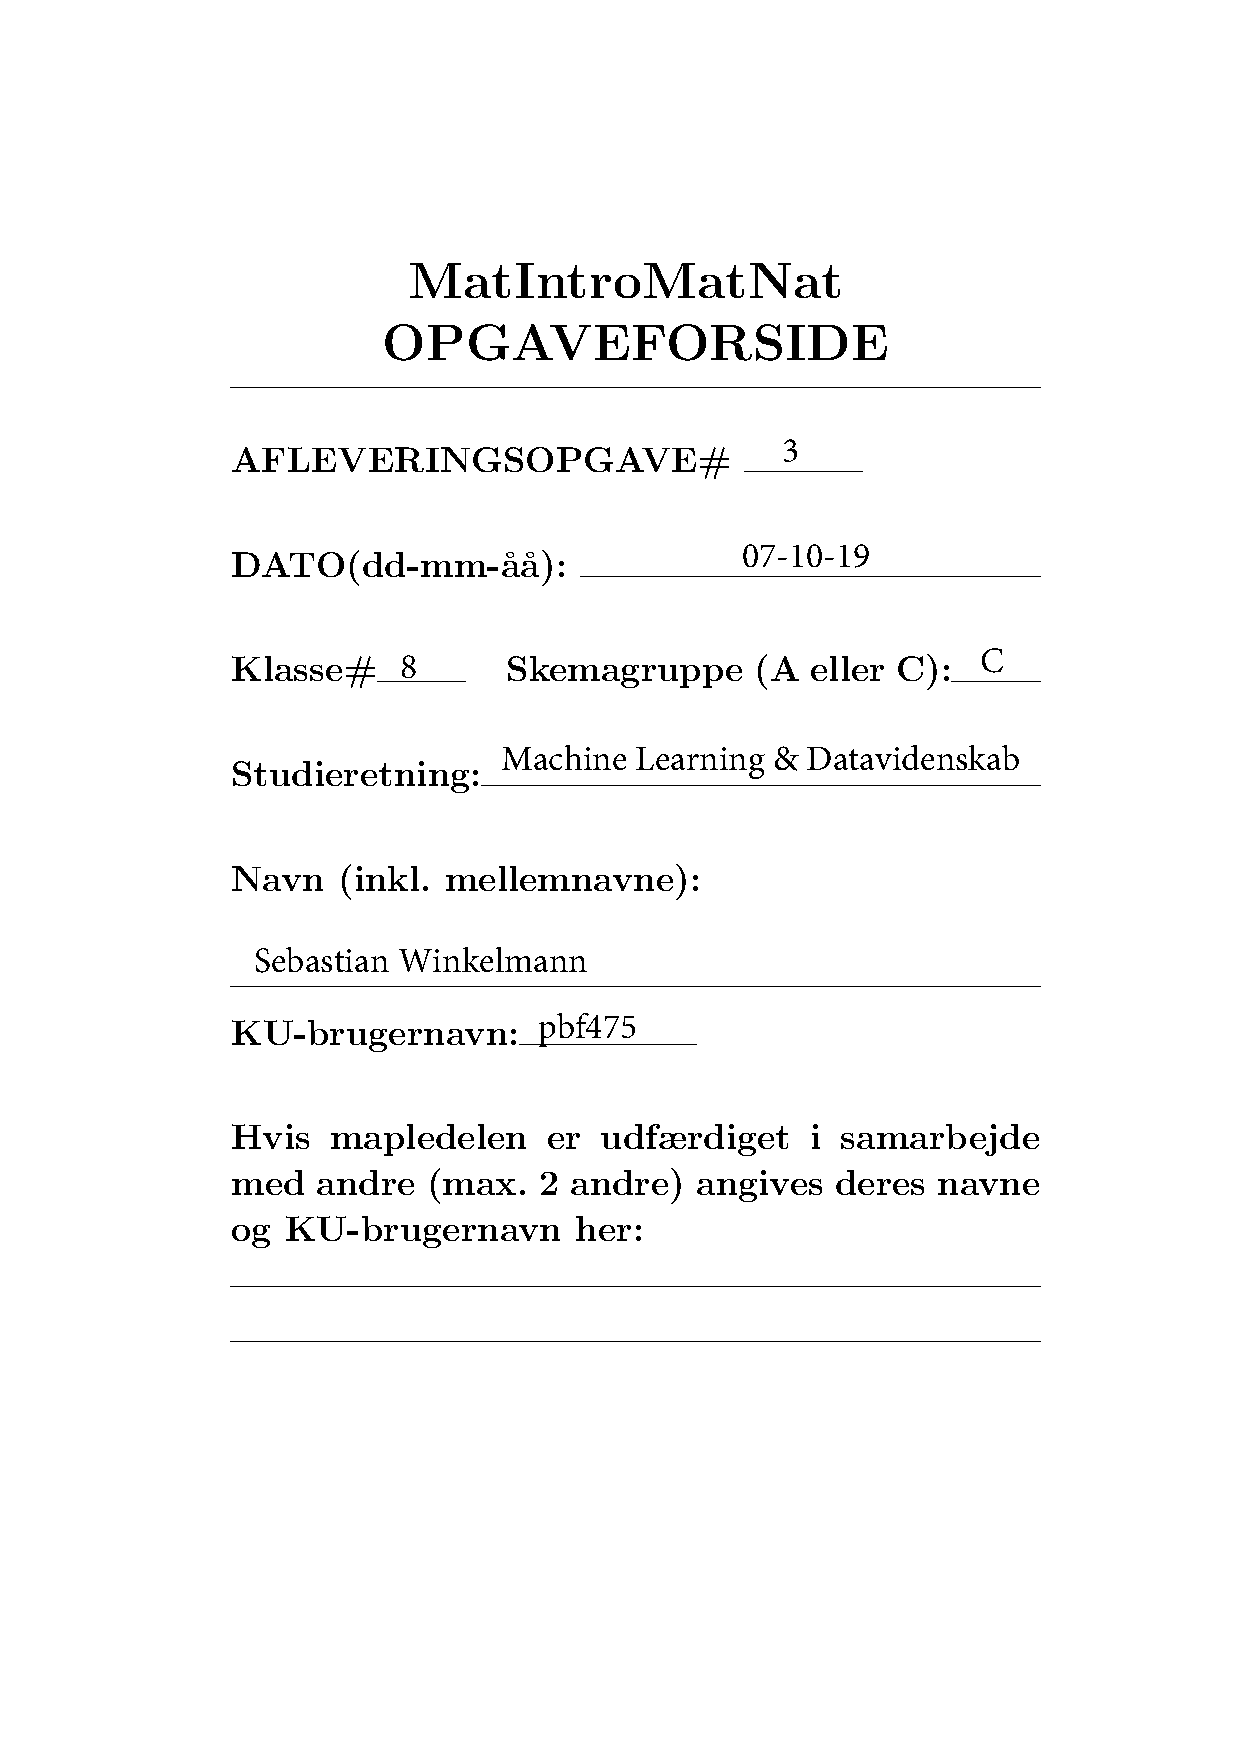
\includepdf{forside.pdf}
\setcounter{chapter}{3}
\section{}
\textit{Betragt funktionen $f(x,y)=\sqrt{5xy-2y^2}$}.
\subsection{Bestem definitionsmængden $D_f$. Skitser $D_f$ i $xy$-planen}
Da man ikke kan tage kvadratroden af et negativt tal gælder der at $2y^2\leq5xy$. Således kan vi isolere for $y$, så $y\leq\frac{5}{2}x$. Vi har altså definitionsmængden for $f$ i den reelle mængde givet ved\begin{equation}
    D_f=\{(x,y)\in\mathbb{R}^2|y\leq\frac{5}{2}x\}
\end{equation}Dette kan meget nemt skitseres ved at at skraveres det område som er mellem ligningen $f(x)=\frac{5}{2}x$ og $x$-aksen:
\begin{figure}[H]
    \centering
    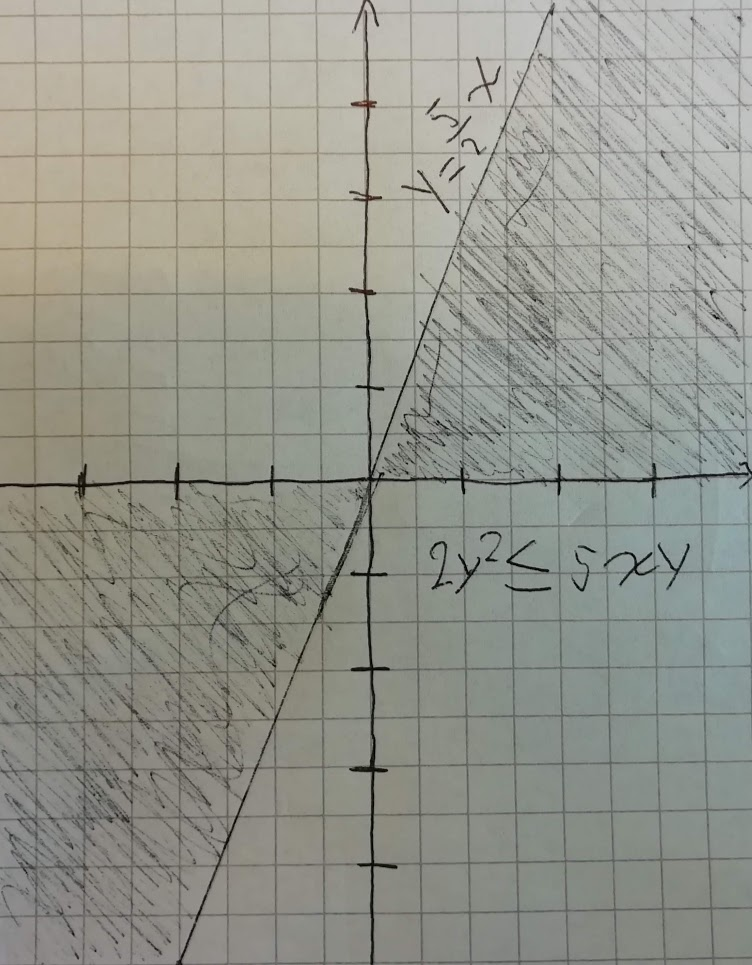
\includegraphics[width=0.3\textwidth]{31aa.png}
\end{figure}
\subsection{Illustration af $f(x,y)$ og uligheden}
\begin{figure}[H]
    \centering
    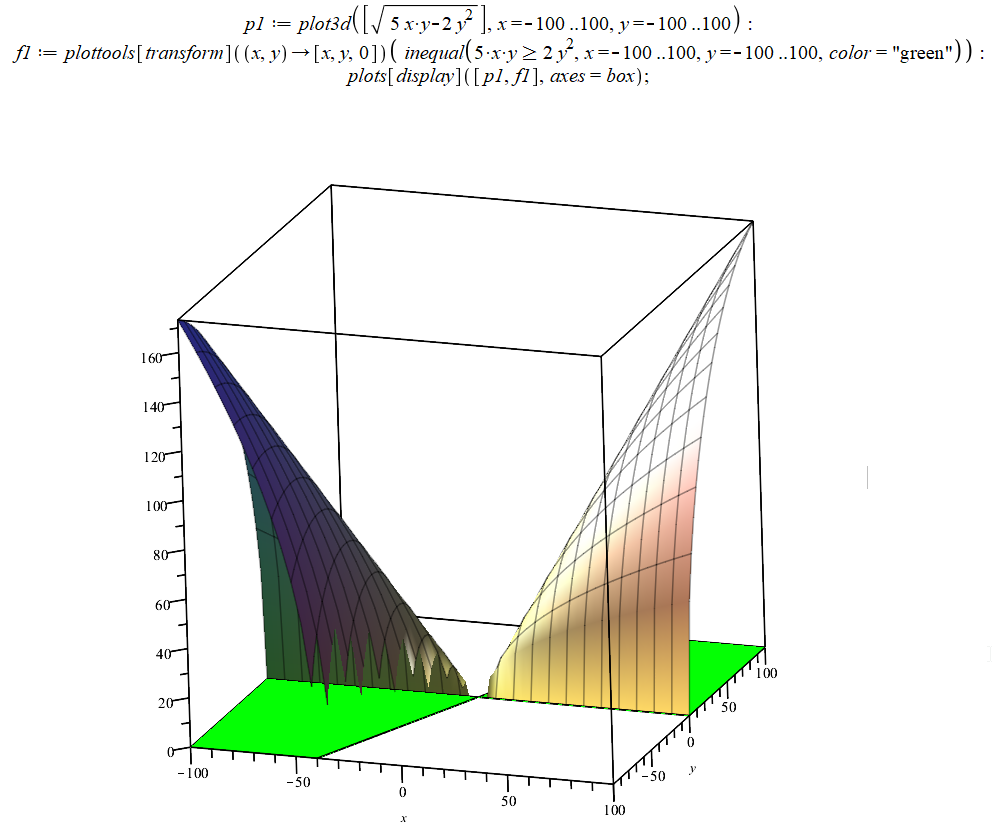
\includegraphics[width=0.5\textwidth]{31b.png}
\end{figure}
\subsection{Grænseværdien}
$$\lim_{h\to0^+}\frac{f(rh,h)}{h},\quad r\geq\frac{2}{5}$$
Lad os indsætte værdierne:
\begin{align*}
    \lim_{h\to0^+}\frac{\sqrt{h^2(5r-2)}}{h}&=\lim_{h\to0^+}\frac{h\sqrt{5r-2}}{h}\\&=\sqrt{5r-2}
\end{align*}
Således er grænseværdien blev fundet ved faktorisering af $h$, til at være $\sqrt{5r-2}$. Bemærk at $h$ er positiv som $h\to0$, derved givet at grænseværdien også er.
\section{$f(x)=2x^4+5x^2-2$}
\subsection{Alle taylorpolynomier omkring $x=1$}
Følger det generelle udtryk for Taylorpolynomium:\begin{equation}
    T_nf(x)=\sum^n_{k=0}\frac{f^{(k)}(a)}{k!}(x-a)^k
\end{equation}{hvor udviklingspunktet er $a$.}
\begin{align*}
    T_0f&=f(1)=2+5-2=5\\
    T_1f&=5+(2\cdot4+5\cdot2-0)\cdot(x-1)=5+18(x-1)\\
    T_2f&=5+18(x-1)+\frac{2\cdot4\cdot3+5\cdot2\cdot1}{2}\cdot(x-1)^2=5+18(x-1)+\frac{34}{2}(x-1)^2\\
    T_3f&=5+18(x-1)+17(x-1)^2+\frac{2\cdot4\cdot3\cdot2+0}{3!}(x-1)^3=5+18(x-1)+17(x-1)^2+\frac{48}{3!}(x-1)^3\\
    T_4f&=T_3f+\frac{2\cdot4\cdot3\cdot2\cdot1}{4!}(x-1)^4=5+18(x-1)+17(x-1)^2+8(x-1)^3+\frac{48}{4!}(x-1)^4\\T_{5\ldots}f&=5+18(x-1)+17(x-1)^2+8(x-1)^3+2(x-1)^4+0+\cdots\\
    &\,\,\,\vdots
\end{align*}
\subsection{Plot}
\begin{figure}[H]
    \centering
    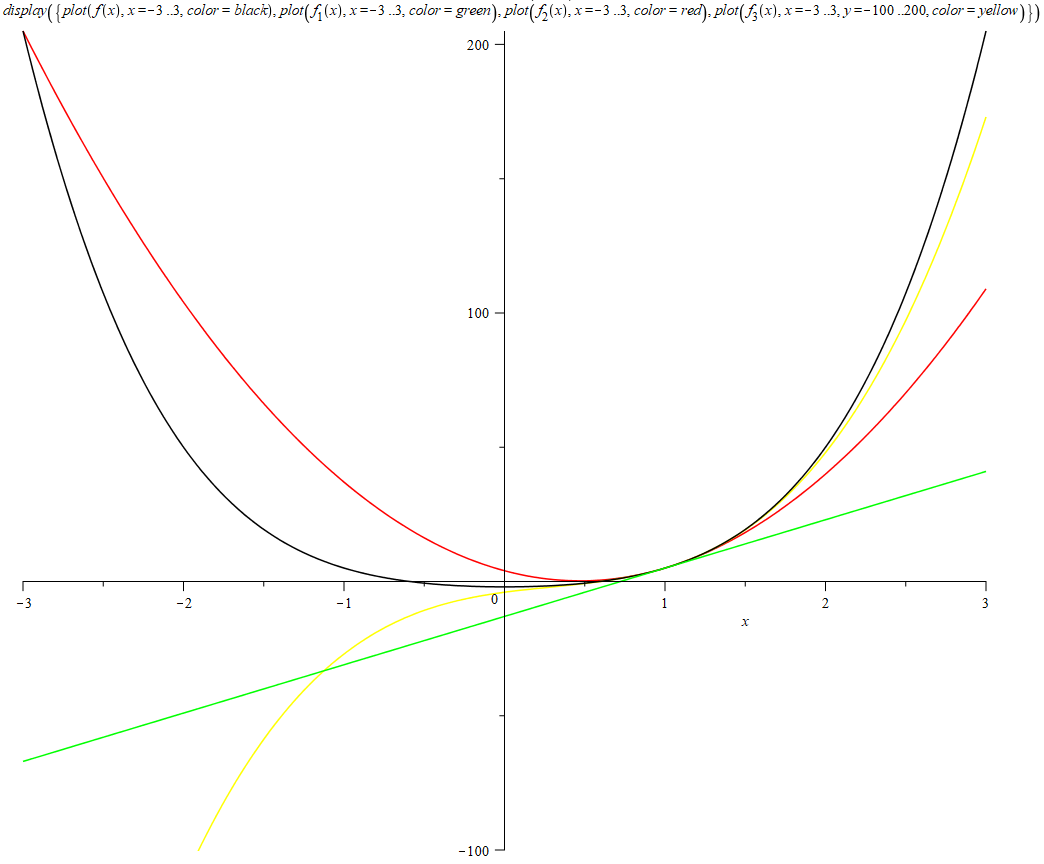
\includegraphics[width=0.53\textwidth]{32b.png}
    \caption{Plot af $f(x)$, \textcolor{green}{$T_1f(x)$}, \textcolor{red}{$T_2f(x)$} og \textcolor{yellow}{$T_3f(x)$}}
\end{figure}{}
\section{Naturlig logaritme}
\textit{Betragt den naturlige logaritmefunktion $f(x)=\ln{x}$, og lad $T_n\ln{}$ være taylorpolynomiet af $n$'te grad omkring $x=1$. Benyt formlen for den $n$-te afledte af $\ln{}$, $f^{(n)}(x)=(-1)^{n-1}(n-1)!x^{-n}$.}
\subsection{Illustrer graferne for $\ln{}, T_9\ln{}$ og $T_{49}\ln{}$ i et fælles koordinatsystem}
\begin{figure}[H]
    \centering
    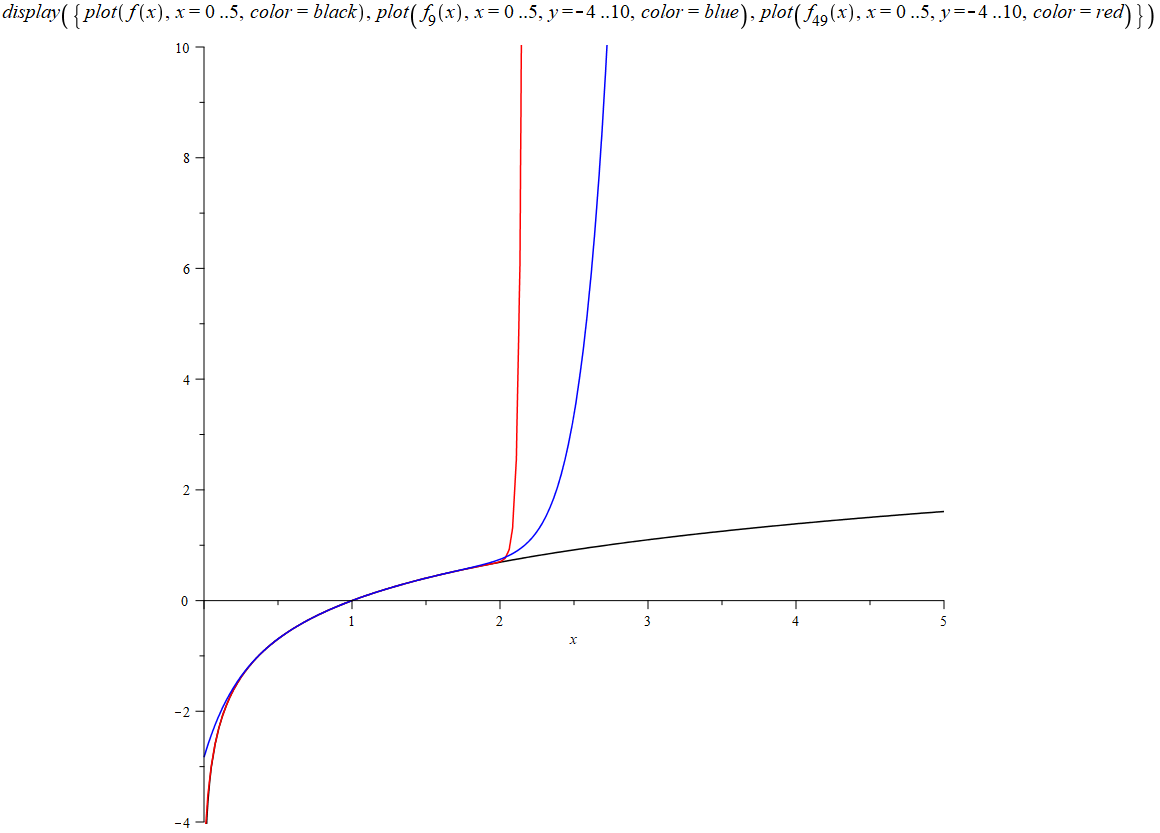
\includegraphics[width=0.8\textwidth]{33a.png}
    \caption{Plot af $f(x)$, \textcolor{blue}{$T_9f(x)$} og \textcolor{red}{$T_{49}f(x)$}}
\end{figure}{}
\subsection{Argumentér ud fra Taylors formel med restled for at}$$|R_n\ln{x}|=|\ln{x}-T_n\ln{x}|\leq\frac{1}{n+1}(x-1)^{n+1}$$\textbf{for $x>1$. Udregn for $x=2$, $x=1.9$ og $x=2.1$, værdien af $T_{49}\ln{x}$ og sammenlign med $\ln{x}$. Kontrollér uligheden ovenfor. Forklar forskellen mellem tilfældene $x<2$ og $x>2$.}

\textbf{11.2.2 Korollar. }Når $f$ og dens $n+1$-afledede er kontinuerlig i intervallet $[a,x]$, lad $M$ være et tal så $|f^{(n+1)}(t)|\leq M$ for alle $t$ mellem $a$ og $x$, da er\begin{equation}
    |R_nf(x)|\leq\frac{M}{(n+1)!}|x-a|^{n+1}
\end{equation}{}
Da $(\ln{x})^{(n+1)}$ og $\ln{x}$ er defineret for alle $x>0$ (og $a=1$), da kan korollaret benyttes. Vi finder værdien for $M$: \begin{align*}
    M&\geq|f^{(n+1)}(t)|=|(-1)^{n+1-1}(n+1-1)!t^{-(n+1)}\\
    M&\geq|(-1)^n n!t^{-(n+1)}|=|t^{-(1+n)}n!|\\
\end{align*}Da det i forvejen er ikke-negativt, kan vi sige $M\geq t^{1-n}n!$ og når $x>1$ kan dette simplificeres til $M\geq n!$ (da $n\to\infty\implies t^{n-1}\to0$ når $t>1$ og at vi kan tage højde for den højeste værdi ved at sige $t=1\implies t^{1-n}=1$, så udtrykket er $n!$). Vi kan sætte dette $M$ ind og simplificere:
$$|R_nf(x)|\leq\frac{n!}{(n+1)!}|x-a|^{n+1}=\frac{1}{n+1}|x-1|^{n+1}$$da $x>1$ vil $x-1>0$:
\begin{equation}
|R_n\ln{x}|=|\ln{x}-T_n\ln{x}|\leq\frac{1}{n+1}(x-1)^{n+1}
\end{equation}
Når $x<2$ følger $T_{49}f$ grafen for $f(x)$ relativt præcist, hvorimod den ved $x>2$ begynder at afvige eksponentielt. Efter $x=2$ bliver afvigelsen enorm, og $T_{49}f$ er herefter voksende i $[2,\infty)$. Da hvert led i taylorpolynomiet har $(x-1)^k$, vil hældningen/afvigelsen stige så snart $x-1>1\implies x>2$. Da der ved et $49$-grads polynomium vil der være værdier opløftet i $49$, hvilket vil give meget stor hældning, modsat $\ln{x}$ som flader ud.
\begin{figure}[H]
    \centering
    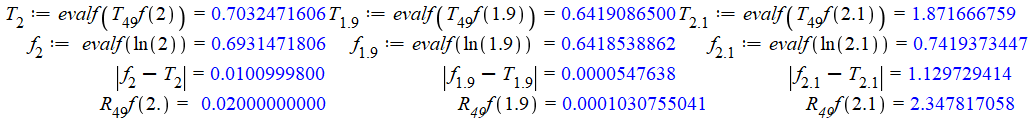
\includegraphics[width=0.8\textwidth]{33b.png}
    \caption{Udregning af $T_{49}f(x)$, $f(x)$, $|\ln{x}-T_n\ln{x}|$ og $\frac{1}{n+1}(x-1)^{n+1}$}
\end{figure}{}
På ovenstående figur kan det tydeligt ses at $T_{49}f$ og $f$ har relativt ens funktionsværdier for $x<2$, men at afvigelsen hurtigt bliver større eftersom $x$ stiger. Det kan desuden konkluderes at den øvre grænse for restleddet holder for alle tre værdier. 
\end{document}